\begin{minipage}[c]{0.4\textwidth}
    \begin{center}
        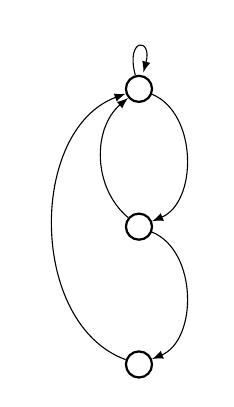
\begin{tikzpicture}[>=latex]
            \node[draw, thick, circle, radius=0.4] (a) at (0,0) {$\textcolor{white}{\cH}\cX\cX\cH\textcolor{white}{\cH}$};
            \node[draw, thick, circle, radius=0.4] (b) at (0,-1.75) {$\textcolor{white}{\cH}\cX\cH\cM\textcolor{white}{\cH}$};
            \node[draw, thick, circle, radius=0.4] (c) at (0,-3.5) {$\textcolor{white}{\cH}\cH\cM\cM\textcolor{white}{\cH}$};
            \draw[->] (a) edge [loop above] node[above] {$\cH$} (a);
            \draw[->] (a) edge [bend left=67.5] node[right] {$\cM$} (b);
            \draw[->] (b) edge [bend left=50] node[left] {$\cH$} (a);
            \draw[->] (b) edge [bend left=67.5] node[right] {$\cM$} (c);
            \draw[->] (c) edge [bend left=70] node[left] {$\cH$} (a);
        \end{tikzpicture}

        (Constraint 1)\\[1pt]
        $\lambda^{\strat}_1 = \overbar{\left<2\right>}^{\text{Kill}}$
    \end{center}
\end{minipage}
\hspace{1cm}
\begin{minipage}[c]{\textwidth}
    \begin{center}
        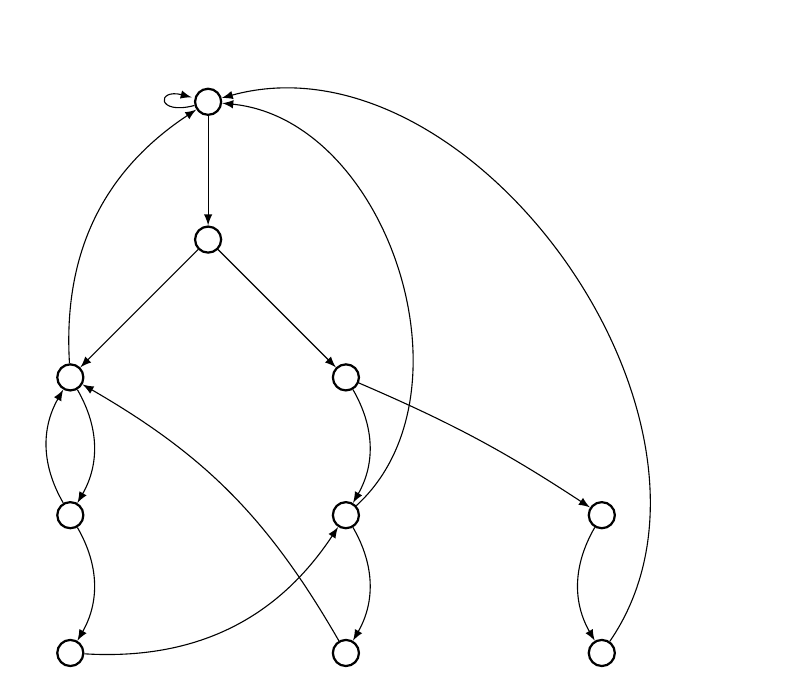
\begin{tikzpicture}[>=latex]
            \node[draw, thick, circle, radius=0.4] (a) at (0,0) {$\cX\cX\cX\cH\cH$};
            \node[draw, thick, circle, radius=0.4] (b) at (0,-1.75) {$\cX\cX\cH\cH\cM$};
            \node[draw, thick, circle, radius=0.4] (c) at (-1.75,-3.5) {$\cX\cX\cH\cM\cH$};
            \node[draw, thick, circle, radius=0.4] (d) at (-1.75,-5.25) {$\cX\cH\cM\cH\cM$};
            \node[draw, thick, circle, radius=0.4] (e) at (-1.75,-7) {$\cH\cM\cH\cM\cM$};
            \node[draw, thick, circle, radius=0.4] (f) at (1.75,-3.5) {$\cX\cH\cH\cM\cM$};
            \node[draw, thick, circle, radius=0.4] (g) at (1.75,-5.25) {$\cX\cH\cM\cM\cH$};
            \node[draw, thick, circle, radius=0.4] (h) at (1.75,-7) {$\cH\cM\cM\cH\cM$};
            \node[draw, thick, circle, radius=0.4] (i) at (5,-5.25) {$\cH\cH\cM\cM\cM$};
            \node[draw, thick, circle, radius=0.4] (j) at (5,-7) {$\cH\cM\cM\cM\cH$};

            \draw[->] (a) edge [loop left] node[left] {$\cH$} (a);
            \draw[->] (a) edge [] node[right] {$\cM$} (b);
            \draw[->] (b) edge node [above] {$\cH$} (c);
            \draw[->] (b) edge node [above] {$\cM$} (f);
            \draw[->] (c) edge [bend left] node [left] {$\cH$} (a);
            \draw[->] (c) edge [bend left] node [right] {$\cM$} (d);
            \draw[->] (d) edge [bend left] node [left] {$\cH$} (c);
            \draw[->] (d) edge [bend left] node [right] {$\cM$} (e);
            \draw[->] (e) edge [bend right] node [below] {$\cH$} (g);
            \draw[->] (f) edge [bend left] node [right] {$\cH$} (g);
            \draw[->] (f) edge [bend left=5] node [above] {$\cM$} (i);
            \draw[->] (g) edge [bend right = 66] node [right] {$\cH$} (a);
            \draw[->] (g) edge [bend left] node [right] {$\cM$} (h);
            \draw[->] (h) edge [bend right = 15] node [above] {$\cH$} (c);
            \draw[->] (i) edge [bend right] node [left] {$\cH$} (j);
            \draw[->] (j) edge [bend right = 70] node [right] {$\cH$} (a);

        \end{tikzpicture}

        (Constraint 2)\\[1pt]
        $\lambda^{\strat}_2 = \overbar{\binom{3}{5}}^{\text{Kill}}$
    \end{center}
\end{minipage}
\hspace{1cm}
\begin{minipage}[c]{0.8\textwidth}
    \begin{center}
        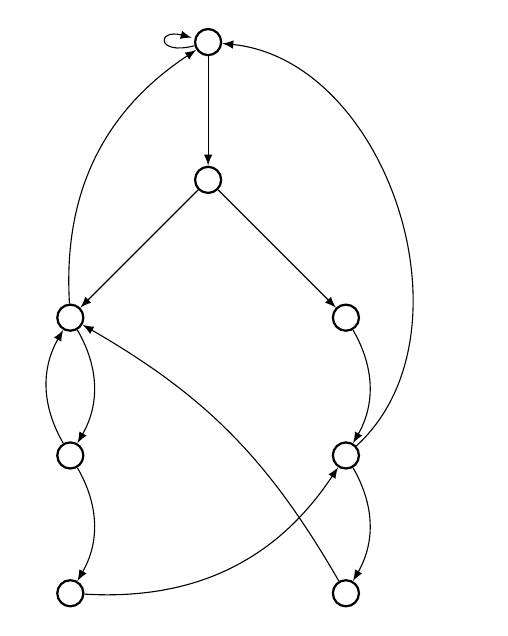
\begin{tikzpicture}[>=latex]
            \node[draw, thick, circle, radius=0.4] (a) at (0,0) {$\cX\cX\cX\cH\cH$};
            \node[draw, thick, circle, radius=0.4] (b) at (0,-1.75) {$\cX\cX\cH\cH\cM$};
            \node[draw, thick, circle, radius=0.4] (c) at (-1.75,-3.5) {$\cX\cX\cH\cM\cH$};
            \node[draw, thick, circle, radius=0.4] (d) at (-1.75,-5.25) {$\cX\cH\cM\cH\cM$};
            \node[draw, thick, circle, radius=0.4] (e) at (-1.75,-7) {$\cH\cM\cH\cM\cM$};
            \node[draw, thick, circle, radius=0.4] (f) at (1.75,-3.5) {$\cX\cH\cH\cM\cM$};
            \node[draw, thick, circle, radius=0.4] (g) at (1.75,-5.25) {$\cX\cH\cM\cM\cH$};
            \node[draw, thick, circle, radius=0.4] (h) at (1.75,-7) {$\cH\cM\cM\cH\cM$};

            \draw[->] (a) edge [loop left] node[left] {$\cH$} (a);
            \draw[->] (a) edge [] node[right] {$\cM$} (b);
            \draw[->] (b) edge node [above] {$\cH$} (c);
            \draw[->] (b) edge node [above] {$\cM$} (f);
            \draw[->] (c) edge [bend left] node [left] {$\cH$} (a);
            \draw[->] (c) edge [bend left] node [right] {$\cM$} (d);
            \draw[->] (d) edge [bend left] node [left] {$\cH$} (c);
            \draw[->] (d) edge [bend left] node [right] {$\cM$} (e);
            \draw[->] (e) edge [bend right] node [below] {$\cH$} (g);
            \draw[->] (f) edge [bend left] node [right] {$\cH$} (g);
            \draw[->] (g) edge [bend right = 66] node [right] {$\cH$} (a);
            \draw[->] (g) edge [bend left] node [right] {$\cM$} (h);
            \draw[->] (h) edge [bend right = 15] node [above] {$\cH$} (c);

        \end{tikzpicture}

        (Result)\\[1pt]
        $\Lambda^{\strat}_0 = \left\{ \lambda^{\strat}_1,\, \lambda^{\strat}_2 \right\}$
    \end{center}
\end{minipage}%}
